%! TeX program = lualatex
\documentclass[a4paper]{article} 

% packages
\usepackage{microtype}      % Slightly tweak font spacing for aesthetics
\usepackage[english]{babel} % Language hyphenation and typographical rules
\usepackage[final, colorlinks = false, urlcolor = cyan]{hyperref} 
\usepackage{changepage}     % adjust margins on the fly
\usepackage{fontspec}

\usepackage{minted}
\usepackage{xcolor}

\usepackage{pgfplots}
\pgfplotsset{width=\textwidth,compat=1.9}

\usepackage{caption}
\newenvironment{code}{\captionsetup{type=listing, skip=0pt}}{}
% \captionsetup{skip=0pt}
% \setlength{\abovecaptionskip}{3pt}
% \setlength{\belowcaptionskip}{5pt}

\usepackage[yyyymmdd]{datetime}
\renewcommand{\dateseparator}{--}
\setmainfont{EB Garamond}
\setmonofont[Scale=MatchLowercase]{Deja Vu Sans Mono}

\usepackage{titlesec}
% \titleformat{\section}{\LARGE\bfseries}{}{}{}[\titlerule]
% \titleformat{\subsection}{\Large\bfseries}{}{0em}{}
% \titlespacing{\subsection}{0em}{-0.7em}{0em}
%
% \titleformat{\subsubsection}{\large\bfseries}{}{0em}{$\bullet$ }
% \titlespacing{\subsubsection}{1em}{-0.7em}{0em}

% margins
\addtolength{\hoffset}{-2.25cm}
\addtolength{\textwidth}{4.5cm}
\addtolength{\voffset}{-3.25cm}
\addtolength{\textheight}{5cm}
\setlength{\parskip}{0pt}
\setlength{\parindent}{0in}
% \setcounter{secnumdepth}{0}

\begin{document}
\hrule \medskip
\begin{minipage}{0.295\textwidth} 
    \raggedright
    \footnotesize 
    Name: Andrew Hayes \\
    E-mail: \href{mailto://a.hayes18@universityofgalway.ie}{\texttt{a.hayes18@universityofgalway.ie}}  \hfill\\   
    ID: 21321503 \hfill
\end{minipage}
\begin{minipage}{0.4\textwidth} 
    \centering 
    \vspace{0.4em}
    \Large 
    \textbf{CT331} \\ 
\end{minipage}
\begin{minipage}{0.295\textwidth} 
    \raggedleft
    \today
\end{minipage}
\medskip\hrule 
\begin{center}
    \normalsize
    Assignment 1: Procedural Programming with C
\end{center}
\hrule

\section{Question 1}
\subsection{Part (A): Code}

\begin{code}
\inputminted[texcl, mathescape, linenos, breaklines, frame=single]{C}{../code/question1/question1.c}
\caption{\texttt{question1.c}}
\end{code}

\begin{figure}[H]
    \centering
    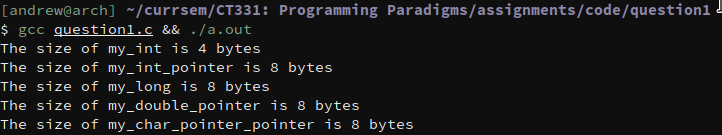
\includegraphics[width=0.8\textwidth]{./images/question1.png}
    \caption{Console Output of \texttt{question1.c}}
\end{figure}

\subsection{Part (B): Comments}
The amount of memory allocated to variables of different types in C is determined at compile-time, and is dependent on the architecture of 
the machine for which it is being compiled and the compiler used.
\begin{itemize}
    \item   On my machine, using GCC, an \verb|int| is allocated 4 bytes. This is the usual amount allocated on both 32-bit and 64-bit systems (my machine being of the 
            latter kind), although older 32-bit systems used 2 bytes for an \verb|int| (the same amount as for a \verb|short|). 
            4 bytes is used even on 64-bit machines to maintain backwards compatibility with older 32-bit architectures.
    \item   An \verb|int*| (a pointer to a variable of type \verb|int|) is allocated 8 bytes on my machine.
            This is because that my machine has a 64-bit architecture, and therefore an address in memory is represented using 64 bits (8 bytes).
            If this were compiled for a 32-bit machine, the size of an pointer would be 4 bytes since addresses are 32-bit.
    \item   A \verb|long| is allocated 8 bytes on my machine. This is because my machine is 64-bit and a \verb|long| is typically 8 bytes in length on such machines.
            On 32-bit machines, a \verb|long| is typically 4 bytes.
    \item   The size of a pointer to a \verb|double| is the same as the size of any other pointer on the same machine; on 64-bit machines, pointers are 8 bytes, and on
            32-bit machines, they are 4 bytes. 
            The type of data to which a pointer points has no effect on the size of the pointer, as the pointer is just a memory address.
    \item   A pointer to a \verb|char| pointer is the same size as any other pointer: 8 bytes on a 64-bit machine and 4 bytes on a 32-bit machine.
            Note: it might be more intuitive to refer to a ``character pointer pointer'' as a pointer to a string in certain situations, as strings are character arrays,
            and an array variable acts as a pointer to the first element in the array. 
\end{itemize}

\section{Question 2}
\begin{code}
\begin{minted}[texcl, mathescape, linenos, breaklines, frame=single]{C}
// returns the number of elements in the list
int length(listElement* list);

// push a new element onto the head of a list and update the list reference using side effects
void push(listElement** list, char* data, size_t size);

// pop an element from the head of a list and update the list reference using side effects
listElement* pop(listElement** list);

// enque a new element onto the head of the list and update the list reference using side effects
void enqueue(listElement** list, char* data, size_t size);  

// dequeue an element from the tail of the list  
listElement* dequeue(listElement* list);  
\end{minted}
\caption{My Additions to \texttt{linkedList.h}}
\end{code}

\begin{code}
\begin{minted}[texcl, mathescape, linenos, breaklines, frame=single]{C}
// returns the number of elements in the list
int length(listElement* list) {
    int length = 0;
    listElement* current = list;

    // traversing the list and counting each element
    while(current != NULL){
        length++;
        current = current->next;
    }

    return length;
}

// push a new element onto the head of a list and update the list reference using side effects
void push(listElement** list, char* data, size_t size) {
    // create the new element
    listElement* newElement = createEl(data, size);

    // handle malloc errors
    if (newElement == NULL) {
        fprintf(stderr, "Memory allocation failed.\n");
        exit(EXIT_FAILURE);
    }

    // make the the new element point to the current head of the list
    newElement->next = *list;

    // make the list reference to point to the new head element 
    *list = newElement;
}


// pop an element from the head of a list and update the list reference using side effects
// assuming that the desired return value here is the popped element, as is standard for POP operations
listElement* pop(listElement** list) {
    // don't bother if list is non existent
    if (*list == NULL) { return NULL; }
;  
    // getting reference to the element to be popped
    listElement* poppedElement = *list;

    // make the the second element the new head of the list -- this could be NULL, so the list would be NULL also
    *list = (*list)->next;

    // detach the popped element from the list
    poppedElement->next = NULL;

    return poppedElement;
}


// enque a new element onto the head of the list and update the list reference using side effects
// essentially the same as push
void enqueue(listElement** list, char* data, size_t size) {
    // create the new element
    listElement* newElement = createEl(data, size);

    // handle malloc errors
    if (newElement == NULL) {
        fprintf(stderr, "Memory allocation failed.\n");
        exit(EXIT_FAILURE);
    }

    // make the the new element point to the current head of the list
    newElement->next = *list;

    // make the list reference to point to the new head element 
    *list = newElement;
} 


// dequeue an element from the tail of the list by removing the element from the list via side effects, and returning the removed item
// assuming that we want to return the dequeued element rather than the list itself, as enqueue returns nothing and uses side effects, so dequeue should also use side effects
listElement* dequeue(listElement* list) {
    // there are three cases that we must consider: a list with 0 elements, a list with 1 element, & a list with >=2 elements

    // don't bother if list is non existent
    if (list == NULL) { return NULL; }

    // if there is only one element in the list, i.e. the head element is also the tail element, just returning this element
    // this means that the listElement pointer that was passed to this function won't be updated
    // ideally, we would set it to NULL but we can't do that since `list` is a pointer that has been passed by value, so we can't update the pointer itself. we would need a pointer to a pointer to have been passed 
    if (list->next == NULL) {
        return list;
    }

    // traversing the list to find the second-to-last element
    listElement* current = list;
    while (current->next->next != NULL) {
        current = current->next;
    }

    // get reference to the element to be dequeued
    listElement* dequeuedElement = current->next;

    // make the penultimate element the tail by removing reference to the old tail
    current->next = NULL;

    return list;
}
\end{minted}
\caption{My Additions to \texttt{linkedList.c}}
\end{code}

\begin{code}
\begin{minted}[texcl, mathescape, linenos, breaklines, frame=single]{C}
    // test length function
    printf("Testing length()\n");
    int l_length = length(l);
    printf("The length of l is %d\n\n", l_length);

    // test push
    printf("Testing push()\n");
    push(&l, "yet another test string", sizeof("yet another test string"));
    traverse(l);
    printf("\n\n");

    // test pop
    printf("Testing pop()\n");
    listElement* popped = pop(&l);
    traverse(l);
    printf("\n\n");

    // Test delete after
    printf("Testing deleteAfter()\n");
    deleteAfter(l);
    traverse(l);
    printf("\n");

    // test enqueue
    printf("Testing enqueue()\n");
    enqueue(&l, "enqueued test string", sizeof("enqueued test string"));
    traverse(l);
    printf("\n");

    // test dequeue
    printf("Testing dequeue()\n");
    dequeue(l);
    traverse(l);
    printf("\n");

    printf("\nTests complete.\n");
\end{minted}
\caption{My Additions to \texttt{tests.c}}
\end{code}

\begin{figure}[H]
    \centering
    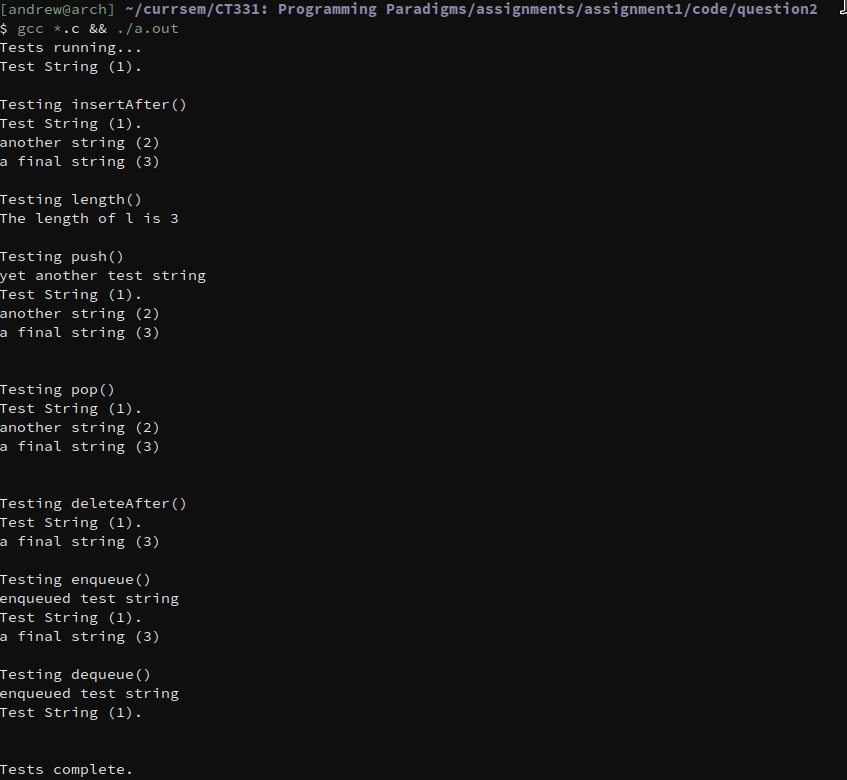
\includegraphics[width=0.9\textwidth]{./images/question2.png}
    \caption{Console Output for Question 2}
\end{figure}

\section{Question 3}
\begin{code}
\inputminted[linenos, breaklines, frame=single]{C}{../code/question3/genericLinkedList.h}
\caption{\texttt{genericLinkedList.h}}
\end{code}

\begin{code}
\inputminted[linenos, breaklines, frame=single]{C}{../code/question3/genericLinkedList.c}
\caption{\texttt{genericLinkedList.c}}
\end{code}

\begin{code}
\inputminted[linenos, breaklines, frame=single]{C}{../code/question3/tests.c}
\caption{\texttt{tests.c}}
\end{code}

\begin{figure}[H]
    \centering
    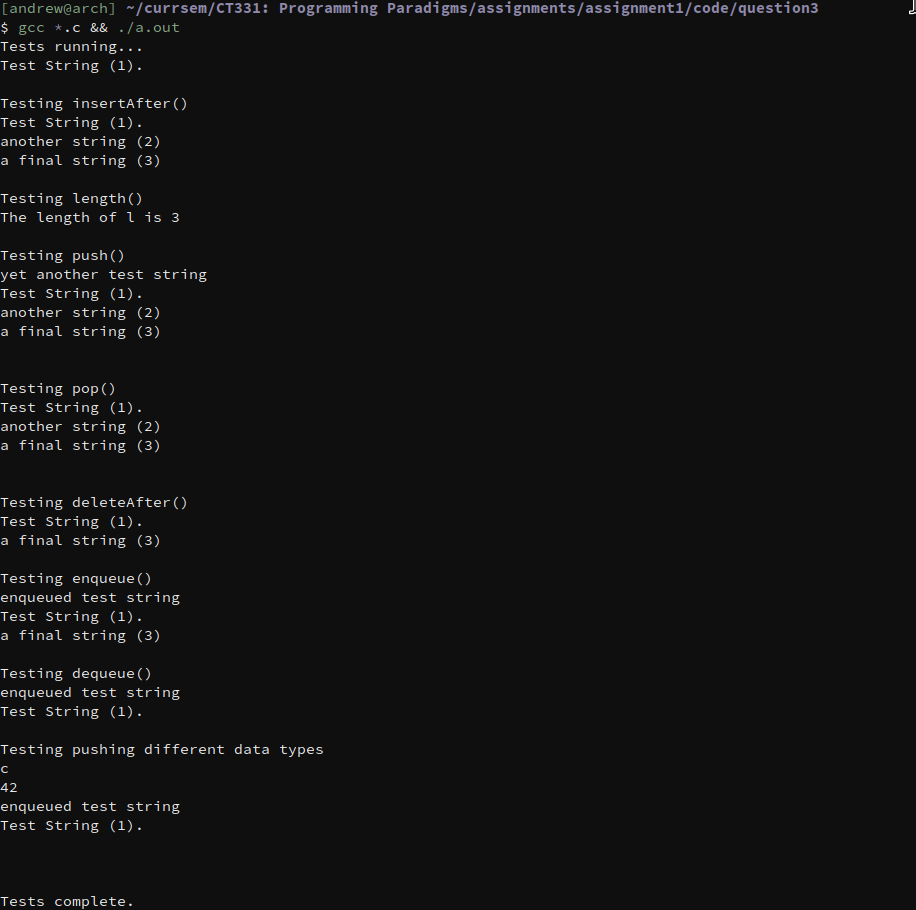
\includegraphics[width=0.9\textwidth]{./images/question3.png}
    \caption{Console Output for Question 3}
\end{figure}

\section{Question 4}
\subsection{Part 1}
Any algorithm for traversing a singly linked list in reverse will always first require traversing the list forwards, and will therefore be \emph{at least} somewhat
less efficient than a forwards traversal.
One of the simplest ways to traverse a linked list in reverse is to use a recursive function.
\begin{code}
\begin{minted}[linenos, breaklines, frame=single]{C}
void reverse_traverse(listElement* current){
    if (current == NULL) { return; }
    reverse_traverse(current->next);
    current->printFunction(current->data);
}
\end{minted}
\caption{Recursive Function to Traverse a Singly Linked List in Reverse}
\end{code}

This is quite inefficient as it requires that the function call for each node persists on the stack until the last node is reached, using a lot of stack memory.
Another approach would be to iteratively reverse the linked list, by making some kind of data structure, linked list or otherwise, that contains the data of the 
original linked list but in reverse, and then iterating over that forwards.  
This would likely be more efficient in terms of memory \& computation.
\\\\
Because traversing a linked list in reverse always requires traversing it forwards first, any reverse algorithm will take at least twice as much memory \& computation
as traversing it forwards, which is $O(n)$.
It will also require that some way of storing the data in reverse in memory, either explicitly with a data, like in the iterative approach, or in the same manner 
as the recursive approach, wherein the data is stored in reverse by the nested structure of the function calls: as each function call returns, the call structure 
is iterated through in reverse.
Therefore, we also have at least $O(n)$ memory usage, as we have to store some sort of reverse data structure.

\subsection{Part 2}
The simplest way in which the structure of a linked list could be changed to make backwards traversal less intensive is to change it from a singly linked list to a 
doubly linked list, i.e. instead of each node in the list containing a pointer to just the next node, make each node contain a pointer to both the next node \& the 
previous node.
The backwards traversal of a doubly linked list is no more intensive than the forwards traversal of a linked list.
The drawback of using a doubly linked list is that it requires slightly more memory per node than a singly linked list, as you're storing an additional pointer 
for every node.





\end{document}
